\section{Opgave 4 - 8 inout NAND using the for loop}
\begin{enumerate}
	\item[1)]
	Vi skriver koden for en 8 input NAND gate ved hjælp af en for løkke i behavioral style som det ses på figur \ref{lst:8innand}.\\
	\begin{lstlisting}[caption={Behavioral style kode en 8 input NAND gate},label={lst:8innand}]
	library ieee;
	use ieee.std_logic_1164.all;
	
	entity inNAND is
	port (input : in std_logic_vector(7 downto 0);
	nand_8 : out std_logic);
	end inNAND;
	
	architecture nand_process of inNAND is
	begin
	comp: process (input)
	begin
	nand_8 <='0'; --default - forudsætter at alle input er høje, og dermed output = 0
	
	for i in 7 downto 0 loop
	if (input(i) = '0') then nand_8 <= '1'; --Hvis bare ét input er lavt, vil output blive 1
	exit;
	end if;
	end loop;
	end process comp;
	end nand_process;
	\end{lstlisting}
	Med en functional simulation ser vi at koden virker efter hensigten, som det ses på figur \ref{fig:8innand}.\\
	\begin{figure}[h]
		\centering
		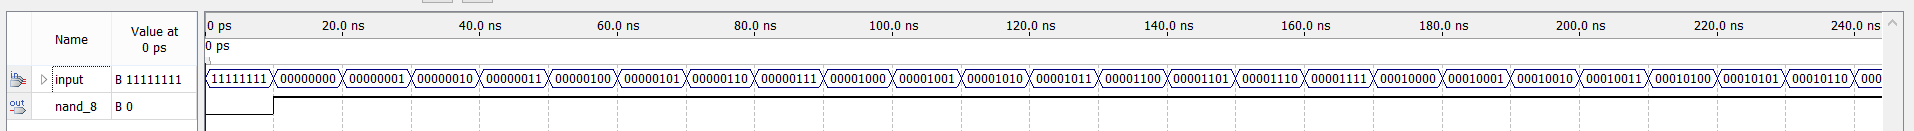
\includegraphics[scale=0.8]{pictures/Oevelse5/opg4/func_sim_8nand.JPG}
		\caption{}
		\label{fig:8innand}
	\end{figure}
\end{enumerate}